\chapter{Sistemas Operativos}

%%%%%%%%%%%%%%%%%%%%%%%%%%%%%%%%%%%%%%%%%%
\section{Sistema de Ficheros}
El \textbf{Sistema de Ficheros} es el componente del sistema operativo encargado de estructurar la información guardada en los dispositivos de almacenamiento. Sus principales funciones son la asignación de espacio a los archivos, la administración del espacio libre y del acceso a los datos guardados.

Existen tres \textbf{tipos} de sistemas de ficheros:
\begin{enumerate}
    \item \textbf{Basados en disco: }están implementados en discos duros. \textit{Ejemplos: Minix, ext2-3-4, FAT, NTFS...}
    \item \textbf{Basados en red (o distribuidos): }se utilizan para acceder a sistemas de ficheros remotos. Independientemente del tipo normalmente se acceden como NFS (Network File System).
    \item \textbf{Basados en memoria (o pseudo): }residen en memoria principal mientras el sistema operativo se está ejecutando.\textit{ Ejemplos: procfs, tmpfs...}
\end{enumerate}
%%%%%%%%%%%%%%%%%%
\subsection{Sistema de Ficheros Virtual}
Un sistema de archivos virtual (VFS) es una capa de abstracción de uno o varios sistemas de ficheros concretos, que permite a las aplicaciones el acceso a diversos tipos de sistemas de archivos concretos, de manera uniforme.


%%%%%%%%%%%%%%%%%%
\subsection{Estructura - ext2}
El sistema de ficheros tiene una tabla donde se almacenan los i-nodos. Un i-nodo almacena información del archivo. La ubicación del fichero es una referencia a un sector del disco donde están todas y cada una de las referencias a los bloques del archivo fragmentado. Estos bloques son de tamaño especificable cuando se crea el sistema de archivos.

%%%%%%%%%%%%%%%%%%
\subsection{Journaling}
La principal desventaja de ext2 es que no implementa el registro por diario (Journaling) que sí poseen sus posteriores versiones ext3 y ext4.\\

El \textbf{journaling} es un mecanismo por el cual un sistema de ficheros puede implementar transacciones. Se basa en llevar un registro (bitácora) en el que se almacena la información necesaria para restablecer los datos afectados por la transacción, en caso de que ésta falle.

\subsubsection{Tipos}
\begin{itemize}
    \item \textbf{Writeback: }no mantiene el orden de actualización entre bloques y la bitácora. Es el más rápido pero no garantiza la integridad en caso de fallo.
    \item \textbf{Ordered: }las actualizaciones de bloques y metadatos se realizan al mismo tiempo en una transacción.
    \item \textbf{Journal mode: }los bloques de datos también se escriben en el archivo de bitácora. Ofrece mayor protección frente a fallos, pero se degrada el rendimiento.
\end{itemize}
%%%%%%%%%%%%%%%%%%%%%%%%%%%%%%%%%%%%%%%%%%
\section{Permisos de Ficheros}
Los permisos de sistemas UNIX se dividen en tres clases, conocidas como usuario, grupo y otros (con frecuencia abreviado UGO, por sus siglas en inglés, User, Group, Others).

\subsubsection{Notación Simbólica}
La \textbf{notación simbólica} permite representar permisos en una serie de 10 caracteres.\\

El \textbf{primer carácter} puede indicar:
\begin{itemize}
    \item \textbf{'-'}: archivo regular.
    \item \textbf{'d'}:	directorio.
    \item \textbf{'l'}:	enlace simbólico.
\end{itemize}
Tras el cual se suceden 3 grupos de 3 caracteres cada uno:
\begin{enumerate}
    \item Lo que el \textbf{propietario} puede hacer.
    \item Lo que los miembros del \textbf{grupo de usuarios} pueden hacer.
    \item Lo que el resto de los \textbf{usuarios no propietarios} pueden hacer.
\end{enumerate}
En cada grupo, cada uno de los tres caracteres representa los permisos de lectura, escritura y ejecución respectivamente:
\begin{enumerate}
    \item 'r' si el bit de lectura está asignado, '-' en caso contrario.
    \item 'w' si el bit de escritura está asignado, '-' en caso contrario.
    \item 'x' si el bit de ejecución está asignado, '-' en caso contrario.
\end{enumerate}

%%%%%%%%%%%%%%%%%%
\section{Tipos de Enlaces}
\begin{itemize}
    \item Un \textbf{enlace físico} es una referencia o puntero a un archivo. Un enlace físico apunta directamente al inodo que contiene la información.\\
    
    Este tipo de ficheros dispone de un \textbf{contador} de enlaces que aumenta o disminuye en función del número de punteros que le referencian. Cuando el puntero llega a 0, el archivo se elimina.
    
    \item Un \textbf{enlace simbólico} no es un puntero que apunta al inodo que contiene los datos, sino que guarda la ruta en la que se encuentra ese inodo. Si se elimina el enlace, no se eliminará el auténtico.
\end{itemize}

\vspace{3cm}
%%%%%%%%%%%%%%%%%%
\section{Cerrojos}
Los cierres de exclusión mutua o cerrojos son un mecanismo de sincronización que limita el acceso a un recurso compartido por varios procesos o hilos en un ambiente de ejecución concurrente, permitiendo así la \textbf{exclusión mutua}.

\subsubsection{El ejemplo del inodoro}
Este mecanismo se puede ver en un ejemplo de la vida real. Supongamos un baño público, donde sólo puede entrar una persona a la vez. Una vez dentro, se emplea un cierre para evitar que entren otras personas.\\

Si otra persona pretende usar el baño cuando está ocupado, deberá quedar esperando a que la persona que entró anteriormente termine. Si más personas llegaran, formarían una cola (del tipo FIFO) y esperarían su turno.
\newpage
%%%%%%%%%%%%%%%%%%%%%%%%%%%%%%%%%%%%%%%%%%
\section{Procesos}
Un \textbf{programa} es un conjunto de instrucciones en código máquina y datos, almacenados en una imagen ejecutable en disco. Un programa es una entidad pasiva.\\

Un \textbf{proceso} es una unidad de actividad que se caracteriza por la ejecución de una secuencia de instrucciones, un estado actual, y un conjunto de recursos del sistema asociados.
\subsection{Estados de un proceso}
\begin{figure}[H]
\centering 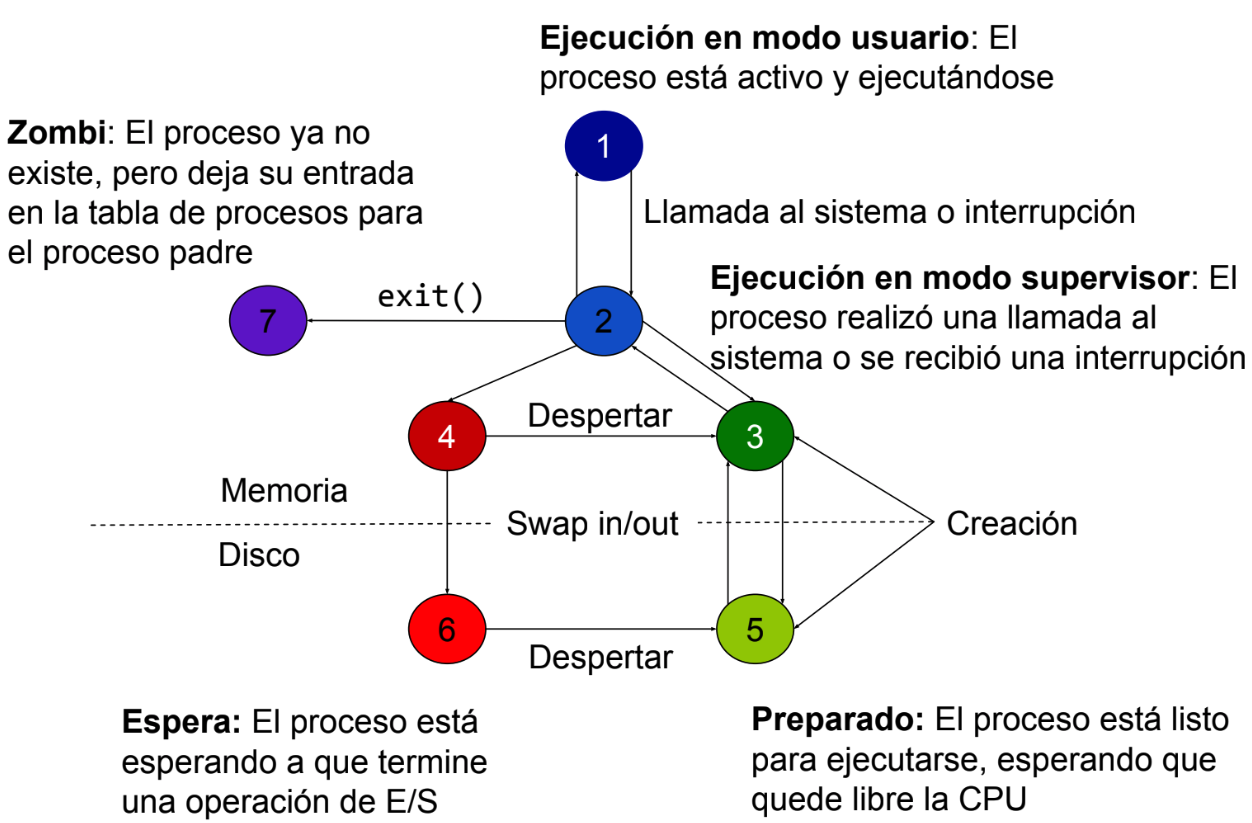
\includegraphics[width=0.9\textwidth]{img/ProcesEstados.png}
\end{figure}

%%%%%%%%%%%%%%%%%%
\subsection{UID}
En sistemas tipo Unix, los usuarios son representados por un identificador de usuario, normalmente abreviado como UID o User ID.
\begin{itemize}
    \item El rango de los valores de los UID varía entre los diferentes sistemas, estando como mínimo comprendidos entre 0 y 32767.
    \item El superusuario debe tener siempre UID 0.
    \item Al usuario nobody siempre se le suele asignar el UID más alto posible (como oposición al superusuario).
\end{itemize}
 Cada proceso maneja dos tipos de UID:
 \begin{itemize}
    \item \textbf{UID real: }identifica al usuario que realmente posee el proceso.
    \item \textbf{UID efectivo: }es el valor que el SO consulta a la hora de tomar decisiones.
 \end{itemize}
 Normalmente el UID real y efectivo tienen el mismo valor, pero cuando ejecutamos un programa del tipo \textit{setuid}, estamos modificando el UID efectivo.
 %%%%%%%%%%%%%%%%%%
\subsection{Permisos}
\textbf{umask} es una orden y una función en entornos POSIX que establece los permisos por defecto para los nuevos archivos y directorios creados por el proceso actual.

Los sistemas Unix modernos permiten que las máscaras se especifiquen de dos modos:
\begin{itemize}
    \item Un permiso por defecto, también llamado máscara simbólica. Por ejemplo, u=rwx,g=rwx,o=
    \item Un número en octal que controla qué permisos se enmascararán (no se establecerán) para cualquier nuevo archivo, por ejemplo, 007.
\end{itemize}


%%%%%%%%%%%%%%%%%%
\subsection{Planificador}
El planificador es un componente esencial en los sistemas operativos. Su función consiste en repartir el tiempo disponible de un microprocesador entre todos los procesos que están disponibles para su ejecución.\\

\subsubsection{Políticas de planificación}
\begin{itemize}
    \item \textbf{SCHED\_OTHER: }Política estándar de tiempo compartido con prioridad 0, que también considera el valor de nice del proceso.
    \item \textbf{SCHED\_FIFO: }Política de tiempo real con prioridades entre 1 y 99, siempre expropiará a los procesos de la clase anterior.
    \item \textbf{SCHED\_RR: }Igual que la anterior, pero a cada proceso se le aplica un cuanto de tiempo de ejecución.
\end{itemize}
\subsubsection{Creación de procesos}
Al hacer \enquote{fork}, se crea un nuevo proceso hijo, con las siguientes características:
\begin{itemize}
    \item El nuevo proceso ejecuta el mismo código que el proceso padre.
    \item Cada proceso dispone de un único identificador
    \item El hijo recibe una copia de los descriptores de los ficheros abiertos por el padre 
    \item El hijo no hereda los cerrojos.
    \item El hijo no hereda las alarmas del padre.
    \item El conjunto de señales pendientes del hijo es nulo.
\end{itemize}
\subsection{Señales}
Una \textbf{señal} es una forma de comunicación entre procesos. En esencia es una notificación asíncrona enviada a un proceso para informarle de un evento. Si se había establecido anteriormente un procedimiento (handler) para tratar esa señal se ejecuta éste, si no se estableció, se ejecuta la acción por defecto para esa señal.
\subsubsection{Tipos de Señales}
\begin{itemize}
    \item Terminación de procesos.
    \item Excepciones.
    \item Llamada de sistema.
    \item Generadas por proceso.
    \item Interacción con el terminal.
    \item Traza de proceso.
\end{itemize}

\begin{comment}
    \subsubsection{Captura}
    Se hace con la llamada a sigaction(señal, acccion, antigua\_accion)
    %Explicar como funciona esta funcion
    \begin{itemize}
        \item sa\_handler
        \item sa\_mask
        \item sa\_flags
    \end{itemize}
    - Si hacemos una llamada al sistema dentro del manejador, es necesario restaurar el valor de errno, justo antes de devolver el control al programa principal.
    %%Programa sa_handler, que acaba cuando hacemos 5 veces ctrl+C
    \begin{lstlisting}[language=C++]
    #include <signal.h>
    #include <stdlib.h>
    
    volatile int count=0;
    
    void handler(int signal){
        count++;
    }
    
    int main(){
        struct sigaction sa;
        int rc;
        
        sa.sa_handler = handler;
        sigemptyset(&sa.sa_mask);
        sa.sa_flags = SA.RESTART;
        rec = sigaction (SIGINT, &sa, NULL);
        if(rc==-1){
            perror("sigaction");
            exit(1);
            //se puede usar tambien exit(EXIT_FAILURE);
        }
        while(count<5);
    }
    \end{lstlisting}
    \subsubsection{Señales de espera}
    La señal sigsuspend.
    \subsubsection{Señales de alarma}
    La señal alarm
    getitimer
    setitimer
    %Y de aqui pasa directamente a tuberias
\end{comment}

\subsection{Tuberías}
Una \textbf{tubería} consiste en una cadena de procesos conectados de forma tal que la salida de cada elemento de la cadena es la entrada del siguiente. Permiten la comunicación y sincronización entre procesos.\\

\textit{Ejemplo: contar las lineas que ocupa ls -l}
\begin{lstlisting}[language=bash,numbers=none]
    $ ls -l | wc -l
\end{lstlisting}

\subsubsection{Tuberías sin nombre (PIPE)}
Las tuberías sin nombre tienen asociado un fichero en memoria principal, por lo tanto, son temporales y se eliminan cuando no están siendo usados ni por productores ni por consumidores. Permiten la comunicación entre el proceso que crea un cauce y procesos hijos tras la creación de la tubería.\\

La comunicación mediante tuberías sin nombre se realiza únicamente entre procesos con relación de parentesco.
\subsubsection{Tuberías con nombre (FIFO)}
Su diferencia respecto a las tuberías sin nombre radica en que el cauce se crea en el sistema de archivos, y por lo tanto no tienen carácter temporal. Se manejan mediante llamadas al sistema (open, close, read y write) como el resto de ficheros del sistema. Permiten la comunicación entre los procesos que usen dicha tubería, aunque no exista una conexión jerárquica entre ellos.\\

Varios procesos pueden abrir la tubería para lectura o escritura, y ambos extremos (de lectura y de escritura) deben abrirse antes de poder intercambiar datos, ya que la apertura se bloquea hasta que se abre el otro extremo.
\subsection{Sincronización de entrada/salida}
Cuando un proceso gestiona varios canales de E/S, debe seleccionar los que están listos en cada momento para realizar la operación.\\

Uno de los métodos para hacerlo es la \textbf{Multiplexación de E/S síncrona}, que consiste en la selección en cada momento del descriptor de fichero que esté listo para realizar la operación de entrada/salida, permitiendo realizarla de forma síncrona.
\begin{comment}
LLamada a select, monitorizar un conjunto de descriptores de ficheros y las señal select se bloquea hasta qu uno de esos descriptores esta listo para ser leido.
Select recibe 3 conjuntos: explicar cabecera.
\end{comment}
\newpage
\section{Sockets}
Socket designa un concepto abstracto por el cual dos programas (posiblemente situados en computadoras distintas) pueden intercambiar cualquier flujo de datos, generalmente de manera fiable y ordenada.\\

Un socket permite el intercambio de datos bidireccional entre procesos cliente y servidor.
\subsection{Tipos de Sockets}
\begin{itemize}
    \item \textbf{SOCK\_STREAM}
    \begin{itemize}
        \item Orientado a conexión, representa un flujo de bytes con entrega ordenada, fiable (retransmisión) y con eliminación de mensajes duplicados.
        \item Comunicación full-duplex.
        \item Flujo de bytes similar a una tubería
        \item Debe establecerse la conexión para poder enviar datos, y se envía la señal SIGPIPE cuando el otro extremo pierde la conexión.
        \item Debe marcarse el principio y final del mensaje (ej. <HTML></HTML>, { “msg”: {...}}).
    \end{itemize}
    
    \item \textbf{SOCK\_DGRAM}
    \begin{itemize}
        \item Basado en datagramas, sin conexión, no confiables, sin entrega ordenada y sin gestión de duplicados.
        \item Comunicación full-duplex.
        \item Envío y recepción de mensajes de longitud máxima fija.
    \end{itemize}
    
    \item \textbf{SOCK\_RAW}
    \begin{itemize}
        \item Permiten acceder a interfaces internos de los protocolos de red que no se exponen directamente vía el API.
        \item Normalmente orientado a datagrama.
    \end{itemize}
\end{itemize}